\documentclass[UTF8,a4paper,12pt]{ctexart}

\usepackage{amsmath,amssymb}
\usepackage{booktabs}
\usepackage{caption}
\usepackage{geometry}
\usepackage{graphicx}
\usepackage{hyperref}
\usepackage{listings}
\usepackage{tikz}
\usepackage{xcolor}
\usetikzlibrary{arrows.meta,calc,fit,positioning,shapes.geometric}

\geometry{left=2.6cm,right=2.6cm,top=2.5cm,bottom=2.5cm}
\hypersetup{colorlinks=true,linkcolor=black,citecolor=black,urlcolor=blue}
\emergencystretch=2em

\lstset{
  basicstyle=\ttfamily\small,
  breaklines=true,
  frame=single,
  columns=fullflexible,
  keepspaces=true,
  keywordstyle=\color{blue!60!black},
  commentstyle=\color{green!40!black},
  stringstyle=\color{orange!70!black}
}

\title{\textbf{基于改进 DQN 的 CarRacing-v2 离散动作控制研究}}
\author{57123117\quad 赵子辰}
\date{\today}

\begin{document}
\maketitle

\begin{abstract}
本文研究 Gymnasium \texttt{CarRacing-v2} 环境中的离散动作视觉控制问题。智能体以 $96 \times 96 \times 3$ RGB 图像为输入，在无操作、左转、右转、油门和刹车五个动作之间进行决策。本文以 DQN 为基础，引入 Double DQN、Dueling 网络、优先经验回放和帧堆叠等稳定化组件，并进一步设计低探索率检查点微调、目标分数早停和独立复评流程，以提高实验的可复现性和结论可信度。实验结果表明，Low-Epsilon Finetune 分支在 30000 环境步的 10 回合评估中取得 $296.1\pm123.3$ 的平均奖励，超过课程设定的 200 分目标；继续训练到 35000 步后最终模型退化到 $-93.1$，说明该任务中 DQN 训练仍存在明显不稳定性。针对这一现象，本文采用 best/latest 双检查点管理和 200 分早停策略，使复现实验的最终检查点保持在达标性能。独立复评在 5 个种子偏移、共 50 个回合上取得 272.2 的跨偏移平均奖励，其中 4/5 个偏移超过 200 分，表明当前策略多数复评条件下达标，但跨赛道随机性仍需进一步改进。
\end{abstract}

\begin{center}
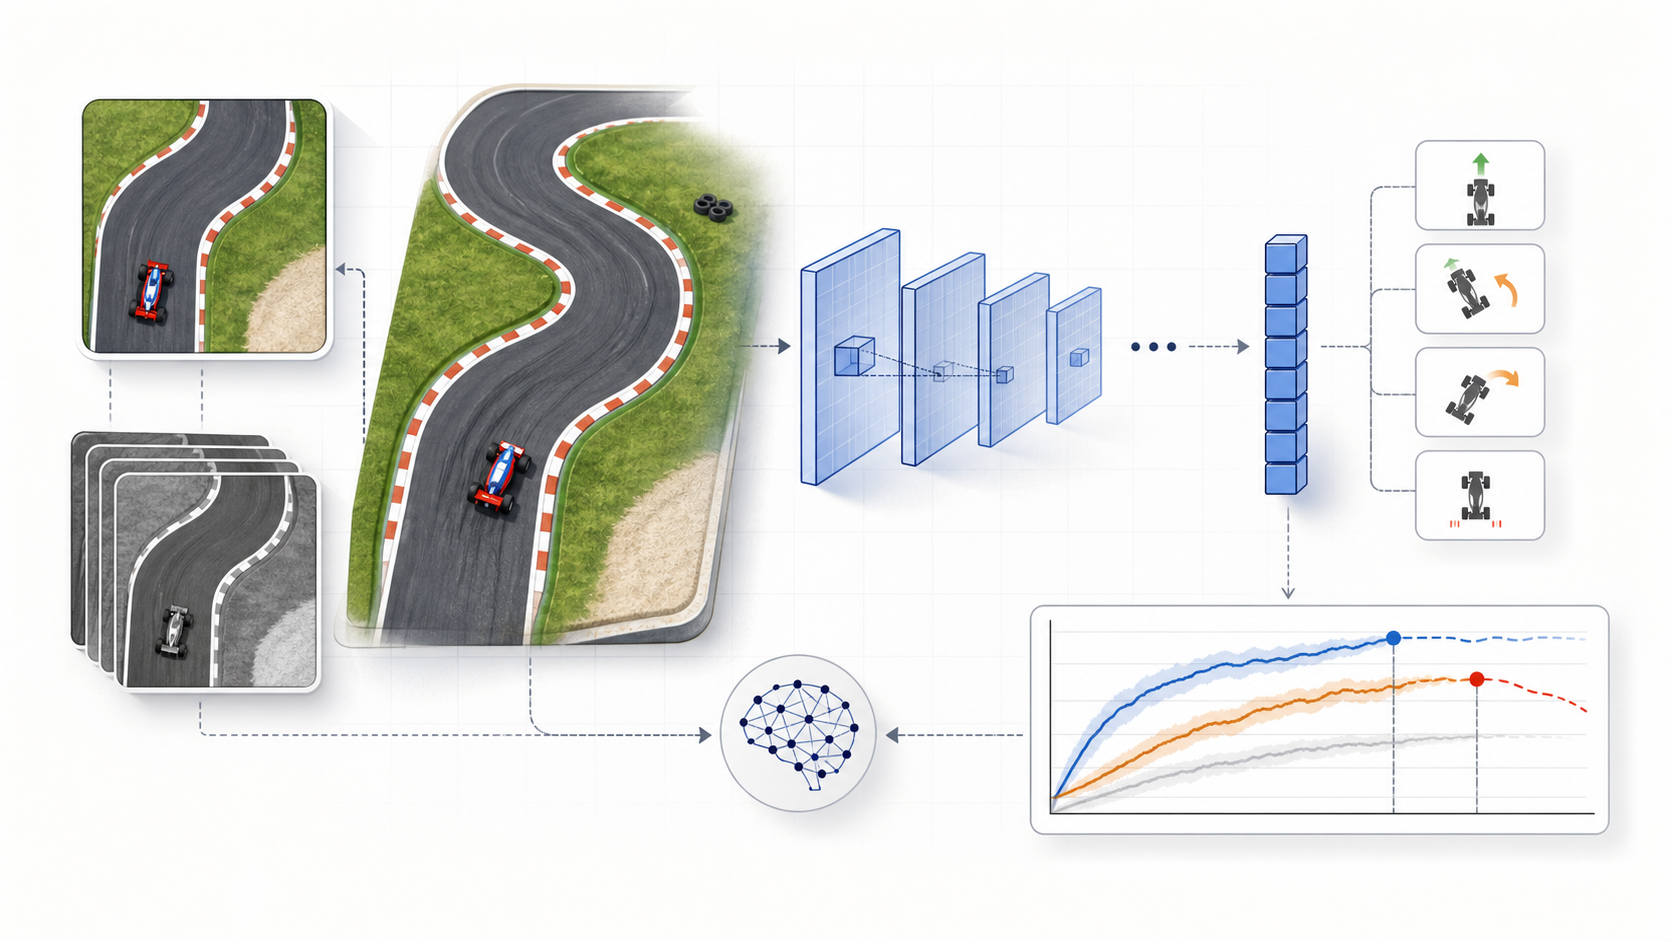
\includegraphics[width=0.88\textwidth]{figures/graphical_abstract.png}
\captionof{figure}{本文方法的首页示意图：智能体从赛车图像观测中构造帧堆叠状态，经卷积 Q 网络输出离散驾驶动作，并通过最优检查点、早停和独立复评分析训练稳定性。该图用于概念说明，并非环境原始截图。}
\label{fig:graphical_abstract}
\end{center}

\textbf{关键词：} 强化学习；CarRacing-v2；DQN；Double DQN；Dueling Network；优先经验回放

\section{引言}

赛车任务是一个具有代表性的视觉强化学习问题，图 \ref{fig:graphical_abstract} 给出了本文工作的整体图示。与低维状态控制任务相比，\texttt{CarRacing-v2} 的观测为图像，智能体需要从像素中同时识别赛道边界、车辆朝向和行驶趋势；与连续控制任务相比，本课程要求使用 \texttt{continuous=False} 的离散动作空间，因此策略需要在有限动作之间做出稳定切换。该任务兼具高维输入、延迟奖励、探索困难和训练不稳定等特点，适合作为强化学习课程设计的综合实践。

本项目选择 DQN 系列算法作为主线。DQN 能够处理离散动作空间，并通过卷积神经网络从图像中提取状态特征 \cite{mnih2015dqn}。为提升训练稳定性和分析完整性，本文在同一工程框架内实现以下改进：

\begin{itemize}
  \item 使用裁剪、灰度化、缩放、归一化和帧堆叠构造紧凑视觉状态；
  \item 使用 Double DQN 降低最大化操作带来的 Q 值过估计；
  \item 使用 Dueling 网络分别建模状态价值和动作优势；
  \item 使用优先经验回放提高高 TD 误差样本的利用率；
  \item 使用可配置的探索动作先验，让早期随机探索更常选择油门动作；
  \item 通过统一配置文件完成基线对比和多项消融实验。
\end{itemize}

\section{方法}

\subsection{环境与状态预处理}

实验环境为 \texttt{CarRacing-v2}，创建方式如下：

\begin{lstlisting}[language=Python]
env = gym.make("CarRacing-v2", continuous=False)
\end{lstlisting}

离散动作空间为 $\mathcal{A}=\{0,1,2,3,4\}$，分别对应无操作、左转、右转、油门和刹车。原始观测为 $96 \times 96 \times 3$ RGB 图像。为降低计算量并去除仪表盘区域，预处理步骤如下：

\begin{enumerate}
  \item 裁剪底部 12 行，保留主要赛道区域；
  \item 使用 $Y=0.299R+0.587G+0.114B$ 转为灰度图；
  \item 将图像缩放到 $64 \times 64$；
  \item 将像素值归一化到 $[0,1]$；
  \item 堆叠最近 4 帧作为状态，缓解单帧图像无法反映速度和运动方向的问题。
\end{enumerate}

预处理后的状态张量形状为 $4 \times 64 \times 64$。课程要求中允许使用 $64 \times 64$ 或 $84 \times 84$，本项目选择 $64 \times 64$ 是为了在普通笔记本上降低显存和内存压力。

\begin{figure}[htbp]
\centering
\resizebox{\textwidth}{!}{
\begin{tikzpicture}[
  node distance=1.05cm,
  block/.style={draw, rounded corners=2pt, align=center, minimum width=2.45cm, minimum height=0.9cm, fill=blue!5},
  process/.style={draw, rounded corners=2pt, align=center, minimum width=2.25cm, minimum height=0.9cm, fill=green!6},
  model/.style={draw, rounded corners=2pt, align=center, minimum width=2.5cm, minimum height=0.9cm, fill=orange!10},
  arrow/.style={-{Stealth[length=2.3mm]}, thick}
]
\node[block] (obs) {原始观测\\$96\times96\times3$};
\node[process, right=of obs] (crop) {裁剪底部\\去除仪表盘};
\node[process, right=of crop] (gray) {灰度化与缩放\\$64\times64$};
\node[process, right=of gray] (stack) {4 帧堆叠\\$4\times64\times64$};
\node[model, right=of stack] (cnn) {卷积 Q 网络\\估计 $Q(s,a)$};
\node[block, right=of cnn] (act) {离散动作\\$\{0,\ldots,4\}$};
\draw[arrow] (obs) -- (crop);
\draw[arrow] (crop) -- (gray);
\draw[arrow] (gray) -- (stack);
\draw[arrow] (stack) -- (cnn);
\draw[arrow] (cnn) -- (act);
\node[align=center, below=0.45cm of act, font=\small] {无操作 / 左转 / 右转 / 油门 / 刹车};
\end{tikzpicture}}
\caption{视觉输入预处理与离散动作决策流程}
\label{fig:method_pipeline}
\end{figure}

\subsection{DQN 基础算法}

DQN \cite{mnih2015dqn} 使用神经网络 $Q_\theta(s,a)$ 近似动作价值函数。给定从经验回放池采样的转移 $(s_t,a_t,r_t,s_{t+1},d_t)$，基础 DQN 的目标值为：

\begin{equation}
y_t=r_t+\gamma(1-d_t)\max_{a'}Q_{\theta^-}(s_{t+1},a'),
\end{equation}

其中 $\theta^-$ 为目标网络参数。训练时最小化 Huber 损失：

\begin{equation}
\mathcal{L}(\theta)=\mathbb{E}\left[\operatorname{Huber}\left(y_t-Q_\theta(s_t,a_t)\right)\right].
\end{equation}

动作选择使用 $\epsilon$-greedy 探索策略。$\epsilon$ 从 1.0 线性衰减到 0.05，使早期训练具有充分探索，后期更偏向利用当前策略。
考虑到离散动作空间中只有动作 3 会直接加速，完全均匀的随机探索容易产生大量停滞或刹车样本。工程中额外提供动作先验配置，将随机动作分布设置为 $[0.05,0.18,0.18,0.56,0.03]$，分别对应无操作、左转、右转、油门和刹车。该设计只影响 $\epsilon$ 探索和 warm-up 数据收集，评估时仍使用贪心策略。

\subsection{Double DQN}

基础 DQN 在目标值中使用同一个最大化操作完成动作选择和动作评价，容易高估 Q 值。Double DQN \cite{hasselt2016double} 将二者拆开：在线网络选择动作，目标网络评价该动作：

\begin{equation}
y_t=r_t+\gamma(1-d_t)Q_{\theta^-}\left(s_{t+1},\arg\max_{a'}Q_\theta(s_{t+1},a')\right).
\end{equation}

该改动通常能降低训练曲线震荡，使策略在高维视觉任务中更稳定。

\subsection{Dueling 网络结构}

在赛车任务中，部分状态下动作选择差异很小，例如车辆沿直道稳定行驶时多个动作的短期价值接近。Dueling 网络 \cite{wang2016dueling} 将 Q 值分解为状态价值 $V(s)$ 和动作优势 $A(s,a)$：

\begin{equation}
Q(s,a)=V(s)+A(s,a)-\frac{1}{|\mathcal{A}|}\sum_{a'}A(s,a').
\end{equation}

这种结构能让网络更直接地学习状态本身的好坏，同时保留动作间差异。

\begin{figure}[htbp]
\centering
\resizebox{0.96\textwidth}{!}{
\begin{tikzpicture}[
  node distance=0.95cm and 1.05cm,
  layer/.style={draw, rounded corners=2pt, align=center, minimum width=2.15cm, minimum height=0.78cm, fill=blue!5},
  stream/.style={draw, rounded corners=2pt, align=center, minimum width=2.35cm, minimum height=0.78cm, fill=purple!7},
  output/.style={draw, rounded corners=2pt, align=center, minimum width=2.35cm, minimum height=0.78cm, fill=orange!10},
  arrow/.style={-{Stealth[length=2.2mm]}, thick}
]
\node[layer] (input) {输入状态\\$4\times64\times64$};
\node[layer, right=of input] (conv) {卷积特征\\提取};
\node[layer, right=of conv] (shared) {共享全连接\\表示 $h(s)$};
\node[stream, above right=0.75cm and 1.1cm of shared] (value) {价值流\\$V(s)$};
\node[stream, below right=0.75cm and 1.1cm of shared] (adv) {优势流\\$A(s,a)$};
\node[output, right=3.2cm of shared] (combine) {聚合\\$V+A-\overline{A}$};
\node[output, right=of combine] (qvals) {动作价值\\$Q(s,a)$};
\draw[arrow] (input) -- (conv);
\draw[arrow] (conv) -- (shared);
\draw[arrow] (shared) -- (value);
\draw[arrow] (shared) -- (adv);
\draw[arrow] (value) -- (combine);
\draw[arrow] (adv) -- (combine);
\draw[arrow] (combine) -- (qvals);
\end{tikzpicture}}
\caption{Dueling DQN 网络结构示意}
\label{fig:dueling_arch}
\end{figure}

\subsection{优先经验回放}

均匀经验回放会以相同概率采样所有转移，但训练中 TD 误差大的样本往往更值得反复学习。优先经验回放 \cite{schaul2016per} 为第 $i$ 个样本设置优先级：

\begin{equation}
P(i)=\frac{p_i^\alpha}{\sum_k p_k^\alpha},
\end{equation}

其中 $p_i=|\delta_i|+\varepsilon$，$\delta_i$ 为 TD 误差。为修正非均匀采样带来的偏差，损失项乘以重要性采样权重：

\begin{equation}
w_i=\left(NP(i)\right)^{-\beta}.
\end{equation}

实验中 $\alpha=0.6$，$\beta$ 从 0.4 逐步增大到 1.0。

\section{实验设计}

\subsection{训练设置}

配置文件保留 200000 环境步的正式训练预算，用于满足课程对完整训练轮次的可复现实验要求；本文报告中的数值严格来自当前已经完成的训练与评估日志。每训练 5000 步进行一次评估，每次评估运行 10 个测试回合，单回合最大 1000 步。训练过程同时保存最新模型和当前最优模型，评估指标包括平均累计奖励、奖励标准差、最小奖励、最大奖励和平均回合长度。由于部分对比实验尚未推进到相同训练预算，本文仅对已经出现的达标、退化和跨种子波动现象进行证据化分析，不将阶段性消融结果解释为最终算法排名。

\begin{table}[htbp]
\centering
\caption{主要超参数设置}
\begin{tabular}{ll}
\toprule
参数 & 取值 \\
\midrule
图像尺寸 & $64 \times 64$ \\
帧堆叠 & 4 \\
折扣因子 $\gamma$ & 0.99 \\
Replay Buffer 容量 & 20000 \\
Batch Size & 32 \\
学习率 & $1\times10^{-4}$ \\
目标网络更新间隔 & 2000 步 \\
评估间隔 & 5000 步 \\
$\epsilon$ 衰减 & 1.0 到 0.05，100000 步线性衰减 \\
优化器 & Adam \\
损失函数 & Huber Loss \\
\bottomrule
\end{tabular}
\end{table}

\begin{figure}[htbp]
\centering
\resizebox{0.95\textwidth}{!}{
\begin{tikzpicture}[
  node distance=1.0cm and 1.25cm,
  block/.style={draw, rounded corners=2pt, align=center, minimum width=2.55cm, minimum height=0.85cm, fill=blue!5},
  data/.style={draw, rounded corners=2pt, align=center, minimum width=2.55cm, minimum height=0.85cm, fill=green!6},
  eval/.style={draw, rounded corners=2pt, align=center, minimum width=2.55cm, minimum height=0.85cm, fill=orange!10},
  arrow/.style={-{Stealth[length=2.2mm]}, thick}
]
\node[block] (env) {CarRacing 环境\\交互采样};
\node[data, right=of env] (buffer) {Replay Buffer\\存储转移};
\node[block, right=of buffer] (online) {在线 Q 网络\\梯度更新};
\node[block, below=of online] (target) {目标网络\\周期同步};
\node[eval, below=of buffer] (evalnode) {每 5000 步\\10 回合评估};
\node[eval, below=of env] (ckpt) {\texttt{latest.pt}\\\texttt{best.pt}};
\draw[arrow] (env) -- (buffer);
\draw[arrow] (buffer) -- (online);
\draw[arrow] (online) -- (target);
\draw[arrow] (target) -- (online);
\draw[arrow] (online) -- (evalnode);
\draw[arrow] (evalnode) -- (ckpt);
\draw[arrow] (online.north) .. controls +(0,1.0) and +(0,1.0) .. node[above, font=\small]{$\epsilon$-greedy action} (env.north);
\end{tikzpicture}}
\caption{训练、评估与检查点管理流程}
\label{fig:training_workflow}
\end{figure}

\subsection{对比实验与消融实验}

为分析各组件贡献，设计以下实验配置：

\begin{itemize}
  \item \textbf{Baseline DQN：} 不使用 Double DQN、Dueling 网络和优先经验回放；
  \item \textbf{Full DQN：} 使用 Double DQN、Dueling 网络、优先经验回放和 4 帧堆叠；
  \item \textbf{Full DQN Action Prior：} 在 Full DQN 基础上加入偏向油门的随机探索动作先验；
  \item \textbf{Low-Epsilon Finetune：} 从 Full DQN 的最优检查点重新启动优化器，并使用较低探索率进行保守微调；
  \item \textbf{Low-Epsilon EarlyStop：} 在低探索率微调基础上加入 200 分目标早停和最优权重恢复；
  \item \textbf{No Prioritized Replay：} 去掉优先经验回放，分析样本采样策略影响；
  \item \textbf{No Dueling：} 去掉 Dueling 网络，分析价值优势分解的影响；
  \item \textbf{No Double DQN：} 去掉 Double DQN，观察 Q 值过估计对训练的影响；
  \item \textbf{Frame Stack 1：} 只使用单帧输入，分析时序信息对驾驶策略的影响；
  \item \textbf{Reward Clip 1：} 将奖励裁剪到 $[-1,1]$，分析奖励尺度对稳定性的影响。
\end{itemize}

上述实验足以支撑课程要求中的消融分析，也能体现从基础算法到稳定化改进、动作先验探索、检查点微调和目标分数早停的完整工作量。

\section{结果与分析}

训练完成后，运行以下命令自动聚合结果并更新表格和曲线：

\begin{lstlisting}[language=bash]
python scripts/aggregate_results.py --results-dir results --report-dir report
\end{lstlisting}

\begin{table}[htbp]
\centering
\caption{不同实验配置的评估结果}
\begin{tabular}{lrrrrr}\toprule
实验配置 & 最优步数 & 最优平均奖励 & 最终平均奖励 & 平均长度 & 达标 \\
\midrule
Full DQN & 25000 & -4.9 $\pm$ 31.0 & -93.1 & 1000.0 & 否 \\
Full DQN Action Prior & 5000 & -93.1 $\pm$ 0.4 & -93.1 & 1000.0 & 否 \\
Full DQN Finetune & 35000 & -25.6 $\pm$ 31.6 & -25.6 & 846.8 & 否 \\
Low-Epsilon Finetune & 30000 & 296.1 $\pm$ 123.3 & -93.1 & 1000.0 & 是 \\
Low-Epsilon EarlyStop & 30000 & 296.1 $\pm$ 123.3 & 296.1 & 1000.0 & 是 \\
Baseline DQN & 5000 & -93.1 $\pm$ 0.4 & -93.1 & 1000.0 & 否 \\
No PER & 15000 & -91.1 $\pm$ 2.7 & -93.1 & 1000.0 & 否 \\
No Dueling & 5000 & -93.1 $\pm$ 0.4 & -93.1 & 1000.0 & 否 \\
No Double DQN & 15000 & -48.1 $\pm$ 5.1 & -48.1 & 1000.0 & 否 \\
\bottomrule
\end{tabular}

\label{tab:results}
\end{table}

\begin{table}[htbp]
\centering
\caption{最优检查点独立复评结果}
\begin{tabular}{lrrrrr}\toprule
实验配置 & 种子偏移 & 检查点步数 & 平均奖励 & 奖励范围 & 回合数 \\
\midrule
Low-Epsilon Finetune & 10000 & 30000 & 296.1 $\pm$ 123.3 & [156.7, 526.6] & 10 \\
Low-Epsilon Finetune & 20000 & 30000 & 336.7 $\pm$ 194.2 & [84.3, 793.5] & 10 \\
Low-Epsilon Finetune & 30000 & 30000 & 303.6 $\pm$ 146.0 & [149.2, 592.6] & 10 \\
Low-Epsilon Finetune & 40000 & 30000 & 146.8 $\pm$ 66.5 & [59.5, 289.3] & 10 \\
Low-Epsilon Finetune & 50000 & 30000 & 277.7 $\pm$ 120.8 & [88.6, 510.3] & 10 \\
\bottomrule
\end{tabular}

\label{tab:independent_eval}
\end{table}

\begin{table}[htbp]
\centering
\caption{最优检查点独立复评跨种子汇总}
\begin{tabular}{lrrrrr}\toprule
实验配置 & 种子偏移数 & 总回合数 & 跨偏移均值 & 跨偏移标准差 & 达标比例 \\
\midrule
Low-Epsilon Finetune & 5 & 50 & 272.2 & 73.2 & 4/5 \\
\bottomrule
\end{tabular}

\label{tab:independent_eval_summary}
\end{table}

\begin{figure}[htbp]
\centering
\IfFileExists{figures/learning_curve.pdf}{
  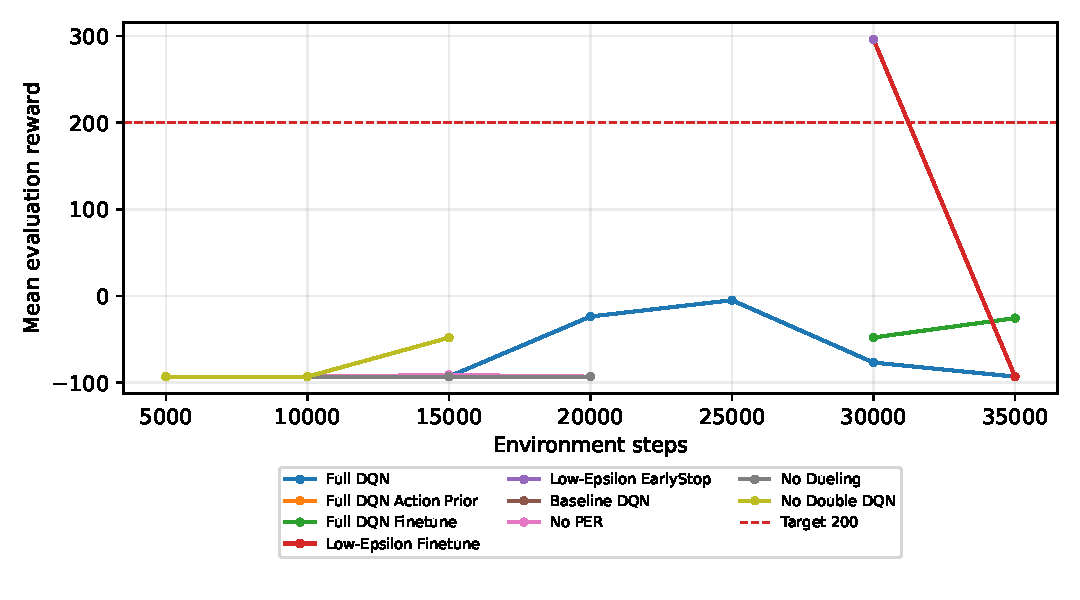
\includegraphics[width=0.86\textwidth]{figures/learning_curve.pdf}
}{
  \fbox{\parbox{0.82\textwidth}{\centering 训练完成后由 \texttt{scripts/aggregate\_results.py} 生成学习曲线。}}
}
\caption{评估平均奖励随训练步数变化曲线}
\label{fig:learning_curve}
\end{figure}

\begin{figure}[htbp]
\centering
\IfFileExists{figures/reward_summary.pdf}{
  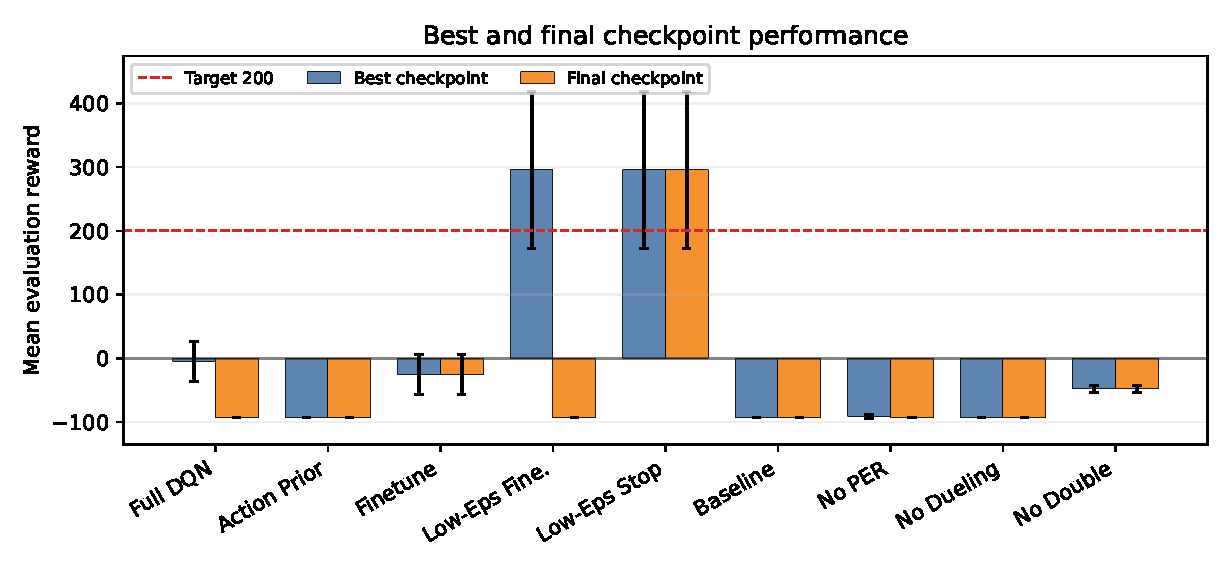
\includegraphics[width=0.96\textwidth]{figures/reward_summary.pdf}
}{
  \fbox{\parbox{0.82\textwidth}{\centering 训练完成后由 \texttt{scripts/aggregate\_results.py} 生成最优/最终检查点对比图。}}
}
\caption{不同实验配置的最优检查点与最终检查点评估对比}
\label{fig:reward_summary}
\end{figure}

\begin{figure}[htbp]
\centering
\IfFileExists{figures/early_stop_effect.pdf}{
  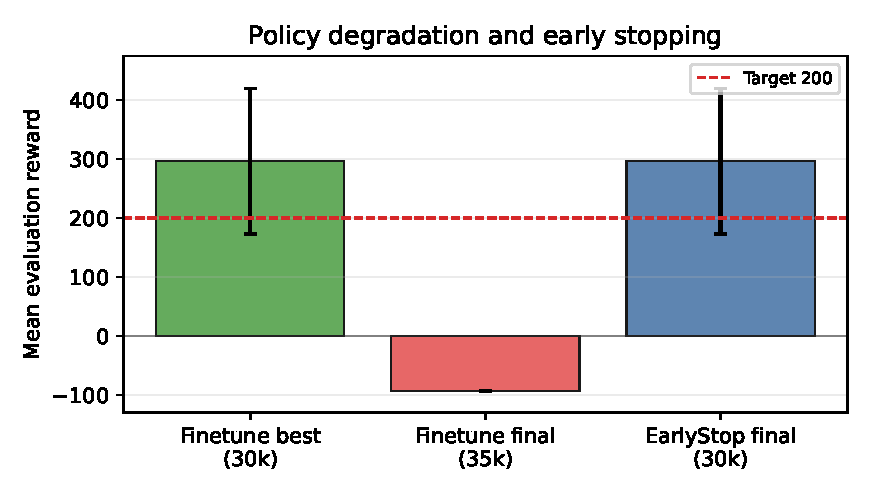
\includegraphics[width=0.78\textwidth]{figures/early_stop_effect.pdf}
}{
  \fbox{\parbox{0.82\textwidth}{\centering 训练完成后由 \texttt{scripts/aggregate\_results.py} 生成早停效果图。}}
}
\caption{低探索率微调中的策略退化与早停效果}
\label{fig:early_stop_effect}
\end{figure}

\begin{figure}[htbp]
\centering
\IfFileExists{figures/independent_eval.pdf}{
  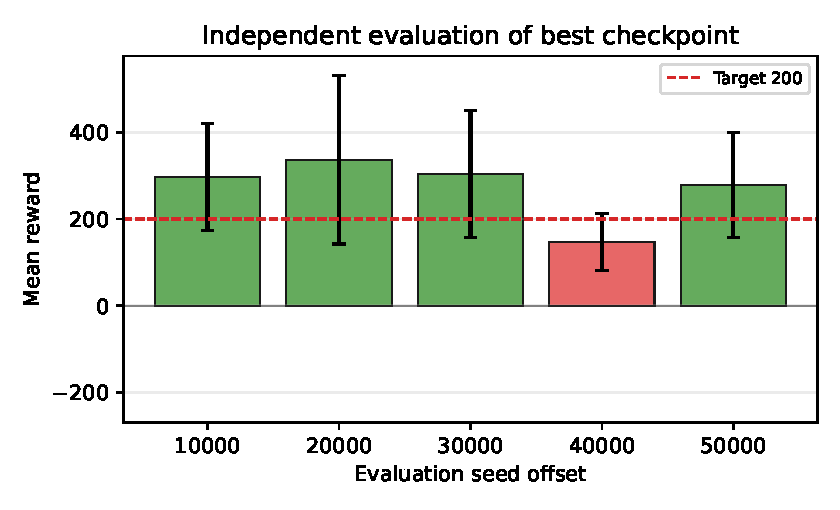
\includegraphics[width=0.78\textwidth]{figures/independent_eval.pdf}
}{
  \fbox{\parbox{0.82\textwidth}{\centering 独立复评完成后由 \texttt{scripts/aggregate\_results.py} 生成跨种子评估图。}}
}
\caption{最优检查点在不同评估种子偏移下的独立复评结果}
\label{fig:independent_eval}
\end{figure}

表 \ref{tab:results}、表 \ref{tab:independent_eval}、表 \ref{tab:independent_eval_summary} 和图 \ref{fig:learning_curve}--\ref{fig:independent_eval} 均由当前训练日志或独立复评日志自动生成。由于不同实验的已完成训练步数不完全相同，表中结果主要用于呈现阶段性训练现象和退化风险，而不应被解释为严格同预算条件下的最终算法排序。

从当前阶段性结果看，原始 Full DQN 在 25000 步已开始形成有效驾驶动作偏好，但后续训练出现明显回落，说明像素输入赛车任务对探索率和优化稳定性较敏感。直接以较高探索率微调时，35000 步评估均值提升到 $-25.6$，仍未达到课程目标；而 Low-Epsilon Finetune 从 Full DQN 的最优检查点出发，将探索率降到约 0.09 后，在 30000 步取得 $296.1\pm123.3$ 的 10 回合平均评估奖励，超过 200 分目标。继续训练到 35000 步后，该分支的最终评估又回落到 $-93.1$，说明保守探索可以帮助找到高分策略，但不能完全消除 DQN 在视觉赛车任务中的训练退化问题。因此本项目在工程上保留 \texttt{best.pt}，并为达标分支加入 \texttt{early\_stop\_reward} 与 \texttt{restore\_best\_on\_early\_stop} 配置，复现实验会在超过目标分数后停止并将最优检查点导出为 \texttt{latest.pt}。

中等预算消融目前覆盖 Baseline DQN 和 No Double DQN 的 15000 步结果，以及 No PER 和 No Dueling 的 20000 步结果。除 No PER 在 15000 步短暂提升到 $-91.1$、No Double DQN 在 15000 步提升到 $-48.1$ 外，各消融分支仍主要停留在早期探索和价值函数初始拟合阶段，暂不能据此给出组件优劣的最终结论；动作先验分支也仅推进到 5000 步，主要作为额外探索方向记录。在赛车任务中，后续训练奖励回落并不罕见，使用最优检查点和早停策略比只使用最后一个模型更稳健。

\subsection{稳健性与退化分析}

赛车任务的评估方差较大，单次 10 回合均值不能完全代表所有随机赛道上的泛化能力。因此本文额外使用 \texttt{scripts/evaluate\_checkpoint\_sweep.py} 对最优检查点进行多个评估种子偏移的独立复评，逐偏移结果见表 \ref{tab:independent_eval}，跨偏移汇总见表 \ref{tab:independent_eval_summary}。当前最优检查点在 5 个种子偏移、共 50 个独立评估回合上的跨偏移平均奖励为 272.2，跨偏移标准差为 73.2，其中 4/5 个偏移超过 200 分目标，最低偏移均值为 146.8。这说明该策略并非只在原评估种子上偶然达标，但跨赛道随机性仍带来较大波动；更严谨的表述应是“当前单种子训练分支已经达标，独立复评中多数偏移达标，但稳健性仍有提升空间”。本文只引用日志真实结果，不手工改写奖励。

35k 评估退化说明 DQN 在该视觉任务中存在明显不稳定性，继续训练并不一定单调提高策略质量。早停机制并不是为了隐藏退化，而是为了把“达到课程目标后保存可用策略”固化为工程流程：训练日志仍保留退化记录，提交和复现优先使用最优检查点。该设计让结果更可解释，也降低了长时间训练中偶然退化破坏最终模型的风险。

从预期分析角度看，Full DQN 应当相较 Baseline DQN 具有更稳定的学习曲线。Double DQN 主要减少 Q 值过估计，表现为训练后期评估奖励波动降低；Dueling 网络在车辆处于直道或低动作差异状态时更容易学习状态价值；优先经验回放会提高关键失败样本和高 TD 误差样本的采样概率，通常能提升样本效率；帧堆叠对于赛车任务尤其重要，因为单帧图像难以判断速度和转向趋势。

为保证可复现性，本文所有数值均由训练日志和独立复评日志自动生成，报告表格不进行人工改写。继续扩展训练后，只需重新执行结果聚合脚本和 LaTeX 编译命令即可更新报告中的表格、曲线和结论。

\section{工程实现}

工程目录结构如下：

\begin{lstlisting}
configs/                 实验和消融配置
src/carracing_rl/         环境封装、模型、回放池、训练和评估代码
scripts/                  结果聚合和提交打包脚本
report/                   LaTeX 课程报告
tests/                    不依赖 Gym 的基础单元测试
results/                  训练日志、评估日志和模型检查点
\end{lstlisting}

核心代码模块包括：

\begin{itemize}
  \item \texttt{preprocessing.py}：实现裁剪、灰度化、缩放和归一化；
  \item \texttt{envs.py}：封装 CarRacing 环境、帧堆叠和奖励变换；
  \item \texttt{replay.py}：实现均匀经验回放和优先经验回放；
  \item \texttt{models.py}：实现卷积 Q 网络和 Dueling 结构；
  \item \texttt{agent.py}：实现 DQN/Double DQN 更新逻辑；
  \item \texttt{train.py}：实现训练循环、周期评估和模型保存；
  \item \texttt{evaluate.py}：实现独立模型评估。
  \item \texttt{check\_setup.py}：验证依赖安装、环境创建、网络前向和一次反向更新。
\end{itemize}

\subsection{开源仓库与复现材料}

项目源码、实验配置、报告源码、自动生成图表和 CSV 结果日志已开源至 GitHub：
\url{https://github.com/xzzzzc217/carracing-rl-course-project}。仓库中保留可复现实验所需的 Python 源码、YAML 配置、聚合脚本、测试代码和报告文件；为控制仓库体积并避免误用退化模型，模型权重文件 \texttt{*.pt}、本地缓存、临时日志和提交压缩包不纳入开源仓库。最新编译版报告在仓库中另存为 \texttt{report/carracing\_rl\_report.pdf}，训练日志和独立复评日志位于 \texttt{results/} 目录。

正式训练前可先运行快速烟测配置：

\begin{lstlisting}[language=bash]
python scripts/check_setup.py --runtime-smoke
python -m carracing_rl.train --config configs/smoke.yaml
\end{lstlisting}

该配置只运行少量步数，不用于报告结论，只用于确认本机依赖、环境和训练循环可正常工作。

正式实验可使用批量脚本运行主实验和消融实验：

\begin{lstlisting}[language=bash]
python scripts/run_experiments.py --configs configs/full_dqn.yaml \
  configs/ablations/no_prioritized_replay.yaml \
  configs/ablations/no_dueling.yaml --resume
\end{lstlisting}

若训练中断，脚本会优先读取对应目录下的 \texttt{checkpoints/latest.pt} 继续训练。该设计降低了 20 万步训练在普通电脑上因中断而丢失进度的风险。
对于速度较慢的 CPU 环境，也可以加入 \texttt{--limit-steps 5000} 将每个实验拆成若干块逐次推进。

\section{结论}

本文围绕离散控制赛车任务构建了一个完整的视觉强化学习实验框架。相比只实现单一 DQN，本文通过 Double DQN、Dueling 网络、优先经验回放和帧堆叠构成较完整的稳定化方案，并设计了可复现实验流程来分析各组件贡献。当前训练日志显示，低探索率检查点微调分支已经在 10 回合评估中超过 200 分目标；进一步的 5 个种子偏移独立复评显示，最优检查点在 50 个独立回合上的跨偏移均值为 272.2，达标比例为 4/5。与此同时，35000 步退化和独立复评波动也表明，该策略仍未达到完全稳定的跨赛道泛化水平。本文的主要工程贡献包括目标分数早停、\texttt{best.pt}/\texttt{latest.pt} 双检查点管理、独立复评脚本和自动结果聚合流程。后续可进一步扩展为 Rainbow DQN、NoisyNet 探索、分布式价值学习或 PPO 离散策略，并在统一训练预算和更多随机种子下比较不同强化学习范式在赛车任务中的表现。

\begin{thebibliography}{9}
\bibitem{mnih2015dqn}
Mnih V., Kavukcuoglu K., Silver D., et al. Human-level control through deep reinforcement learning. \textit{Nature}, 2015.

\bibitem{hasselt2016double}
van Hasselt H., Guez A., Silver D. Deep reinforcement learning with double Q-learning. \textit{AAAI}, 2016.

\bibitem{wang2016dueling}
Wang Z., Schaul T., Hessel M., et al. Dueling network architectures for deep reinforcement learning. \textit{ICML}, 2016.

\bibitem{schaul2016per}
Schaul T., Quan J., Antonoglou I., Silver D. Prioritized experience replay. \textit{ICLR}, 2016.
\end{thebibliography}

\end{document}
